\documentclass[border=5pt]{standalone}
\usepackage{tikz}
\usepackage{amsmath}
\begin{document}
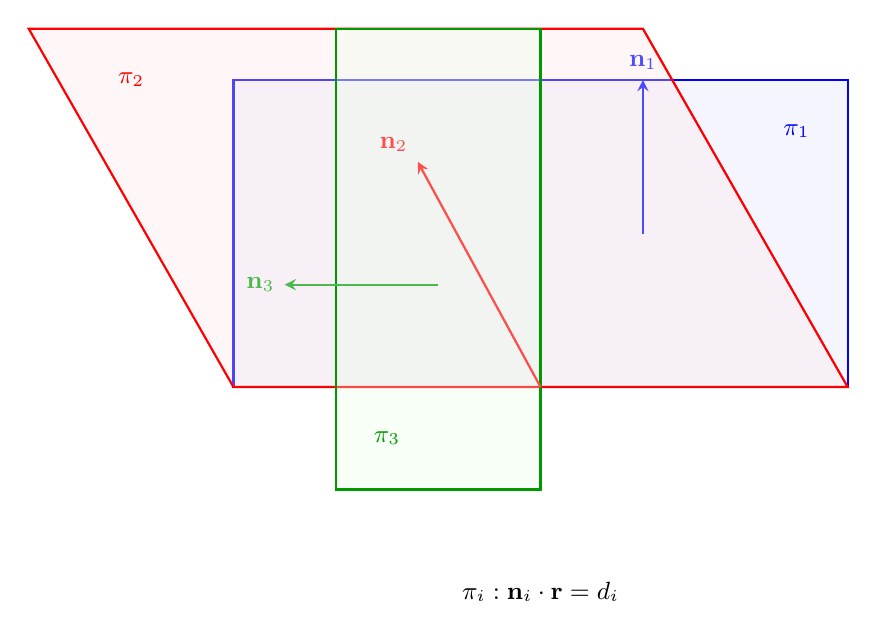
\begin{tikzpicture}[scale=1.3, >=stealth]
  % Three planes relationship

  % Plane 1
  \fill[blue!10, opacity=0.4] (-3,0) -- (3,0) -- (3,3) -- (-3,3) -- cycle;
  \draw[thick, blue] (-3,0) -- (3,0) -- (3,3) -- (-3,3) -- cycle;
  \node[blue, font=\small] at (2.5, 2.5) {$\pi_1$};

  % Plane 2 (tilted)
  \fill[red!10, opacity=0.3] (-3,0) -- (3,0) -- (1,3.5) -- (-5,3.5) -- cycle;
  \draw[thick, red] (-3,0) -- (3,0) -- (1,3.5) -- (-5,3.5) -- cycle;
  \node[red, font=\small] at (-4, 3) {$\pi_2$};

  % Plane 3 (other tilt)
  \fill[green!10, opacity=0.3] (0,-1) -- (0,3.5) -- (-2,3.5) -- (-2,-1) -- cycle;
  \draw[thick, green!60!black] (0,-1) -- (0,3.5) -- (-2,3.5) -- (-2,-1) -- cycle;
  \node[green!60!black, font=\small] at (-1.5, -0.5) {$\pi_3$};

  % Normal vectors
  \draw[->, thick, blue!70] (1, 1.5) -- (1, 3) node[above, font=\small] {$\mathbf{n}_1$};
  \draw[->, thick, red!70] (0, 0) -- (-1.2, 2.2) node[above left, font=\small] {$\mathbf{n}_2$};
  \draw[->, thick, green!60!black!70] (-1, 1) -- (-2.5, 1) node[left, font=\small] {$\mathbf{n}_3$};

  % Formula
  \node[font=\small] at (0, -2) {$\pi_i: \mathbf{n}_i \cdot \mathbf{r} = d_i$};
\end{tikzpicture}
\end{document}
